\begin{center}
    % --- Minipage Sinistra: Matrice di Transizione ---
    \begin{minipage}[c]{0.45\textwidth}
        \centering
        \renewcommand{\arraystretch}{1.5} % Spazio verticale interno alla matrice
        $\begin{pmatrix} 
            1-\epsilon & 0 & \epsilon \\ 
            0 & 1-\epsilon & \epsilon 
        \end{pmatrix}$
    \end{minipage}
    \hfill
    % --- Minipage Destra: Diagramma del Canale ---
    \begin{minipage}[c]{0.45\textwidth}
        \centering
        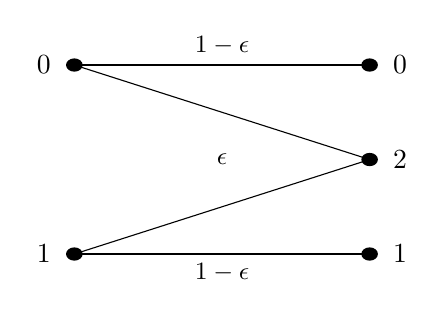
\begin{tikzpicture}[yscale=1.2, xscale=1.5]
            % Nodi di ingresso (Input: 0, 1)
            \node[left=5pt] at (0,0) {$0$}; \fill (0,0) circle (2pt) coordinate (x0);
            \node[left=5pt] at (0,-2) {$1$}; \fill (0,-2) circle (2pt) coordinate (x1);

            % Nodi di uscita (Output: 0, 2, 1)
            \fill (2.5,0) circle (2pt) coordinate (y0); \node[right=5pt] at (2.5,0) {$0$};
            \fill (2.5,-1) circle (2pt) coordinate (y2); \node[right=5pt] at (2.5,-1) {$2$};
            \fill (2.5,-2) circle (2pt) coordinate (y1); \node[right=5pt] at (2.5,-2) {$1$};

            % Collegamenti orizzontali (Successo)
            \draw (x0) -- node[above] {\small $1-\epsilon$} (y0);
            \draw (x1) -- node[below] {\small $1-\epsilon$} (y1);

            % Collegamenti diagonali verso l'uscita di cancellazione '2'
            \draw (x0) -- (y2);
            \draw (x1) -- (y2);
            
            % Etichetta epsilon centrale (Cancellazione)
            \node[fill=white, inner sep=2pt] at (1.25, -1) {\small $\epsilon$};
        \end{tikzpicture}
    \end{minipage}
\end{center}